同じ数列を保持するような、形の異なる二分木( binary tree )は多く存在し得ます。
例えば、ここに数列 1, 1, 2, 3, 5, 8, 13 を保持する2つの二分木があります。

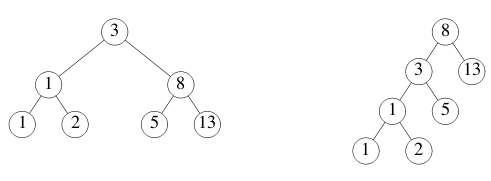
\includegraphics[width=10cm]{tree.png}

2つの二分木が同じ数列を保持しているかどうかを確認する機能は、多くの言語においてかなり複雑です。

シンプルな解決方法を記述するために、Goの並行性( concurrency )とチャネルを利用してみます。

例では、型を以下のように定義している \texttt{tree} パッケージを利用します:

\begin{lstlisting}[numbers=none]
type Tree struct {
    Left  *Tree
    Value int
    Right *Tree
}
\end{lstlisting}

1. \texttt{Walk} 関数を実装してください。

2. \texttt{Walk} 関数をテストしてください。

関数 \texttt{tree.New(k)} は、値( \texttt{k}, \texttt{2k}, \texttt{3k}, ..., \texttt{10k} )
をもつ、ランダムに構造化 (しかし常にソートされています) した二分木を生成します。

新しいチャネル \texttt{ch} を生成し、 \texttt{Walk} を動かしましょう:

\begin{lstlisting}[numbers=none]
go Walk(tree.New(1), ch)
\end{lstlisting}

そして、そのチャネルから値を読み出し、10個の値を表示してください。 それは、 1, 2, 3, ..., 10 という表示になるでしょう。

3. \texttt{Same} 関数を実装してください。 \texttt{t1} と \texttt{t2}
が同じ値を保存しているどうかを判断するため、 \texttt{Walk} を使ってください。

4. \texttt{Same} 関数をテストしてください。

\texttt{Same(tree.New(1), tree.New(1))} は、 \texttt{true} を
返すように、 \texttt{Same(tree.New(1), tree.New(2))} は、 \texttt{false} を
返すようにします。

\texttt{Tree} のドキュメントは
こちら(https:\//\//godoc.org\//golang.org\//x\//tour\//tree\#Tree) です。


